\chapter{Methodology}
In this chapter the iterative work process, data collection, and the technical tools used during development are explained.
\section{Work Process}
% Olika faser:
% Inläsning, hämta grundläggande data, använd färdiga algos, implementera baseline, extend upon baseline
% enklare operationr först, sedan påbörja svårare

The methodology used for the thesis is a mixture of reading prior literature on common compression algorithms, spatial operations, and floating-point representations. Along with data collection and preprocessing, implementing benchmarking and validation environments, and iteratively implementing and evaluating ideas obtained through brainstorming and combining existing literature. When ideas were proposed, the potential gain and estimated implementation complexity were used to rank the development order. Thus, some ideas were never implemented due to time constraints, but the ideas are still documented in the report for future reference.   

A rough overview of the process used during the 20 weeks of the thesis is presented below:
\begin{enumerate}

  \item Look into different sources for open-source map data where the geometrical object format is known. When decided, incorporate the data into an existing geometric framework, such as \emph{Shapely}, and become familiar with the formats. Set up an environment for testing, developing, and evaluating implementations of compression algorithms performing geometric operations on the processed data.
    
  \item Conduct a literature review of compression concepts and encoding of geometries consisting of floating-point coordinates. Investigate what kind of algorithms are suitable for geometrical map data.

  \item Implement one baseline algorithm which can be extended. The baseline should perform the geometric operations by decompressing the whole geometry, and the algorithm should be relevant in the field of maps compression.
  
  \item Change the underlying structure of the baseline to enable unary and binary operations by partial decompression. Performed by iteratively coming up with new ideas, implementing them, and measuring the performance difference between the algorithms in terms of efficiency and storage space.

  \item Examine how the compression ratio can be optimized while preserving the operability, by exploiting the maps domain and applying a combination of known compression strategies. Also, improve execution time by utilizing profiling tools and optimizing the implementation.


\end{enumerate}


\section{Establishing the Baseline}
Due to the significant performance differences between programming languages, such as C and Python, programming language consistency is critical to ensure a fair comparison between implementations. As mentioned in Section \ref{scopeLimit},  the implementation of our compression format is written in Python, and for conducting fair performance assessments, an appropriate baseline was re-implemented in Python. The baseline provides a base for evaluation, and by comparing the relative performance scoring between different implementations, an idea of their general performance can be extrapolated. 

For instance, if implemented in the same programming language, comparing the execution time of a baseline that decompresses an entire geometry with the execution time of an operation-integrated compression format with support for partial decompression, valid data on the performance benefits of partial decompression can be obtained. However, if the operations are done in different languages, the effect of the different languages cannot be controlled.

Nonetheless, there are situations where valuable insights can be gained by comparing operations written in \textit{partially different} languages. If an operation-integrated compression format outperforms the complete operation, which includes decompression and a library function in the baseline, and both use the same programming language for the decompression, despite the possibility that the baseline might utilize a more efficient library function, the operation-integrated compression format demonstrates its superiority by outperforming the baseline in overall time.

\section{Supported Operations}
There exist many operations which can be used to manipulate or extract information from geometries. To narrow the scope of the thesis, the supervisors proposed some operations that are often performed on GIS data. Three distinct operations were chosen as the primary goals of optimization: \emph{bounding box}, \emph{add vertex}, and \emph{intersection} (both \emph{predicate} and \emph{boolean}). The operations are characterized by being \emph{constant}, \emph{modifying}, and \emph{binary} operations, respectively.
\\\\
During meetings with the supervisors, the following unary operations were proposed as interesting and while only a few are in focus for the thesis, the others may be integrated and optimized in future work:
\begin{description}
    \item[Vertex Count] Number of total vertices.
    \item[Area] For polygons, the total area minus the area of the holes.
    \item[Length] Total length for linestrings, circumference for polygons.
    \item[Modify Vertices] Add, remove, edit individual vertices.
    \item[Bounding Box] Returns the corners of the minimum axis-aligned rectangle such that all vertices in the shape are contained.
    \item[Buffering/Scaling] Change the size of the geometry while preserving the center of mass and proportions. 
    \item[Convex Hull] The smallest convex set containing the shape.
    \item[Center of Mass] Average position of all vertices.
    \item[End-Points] For linestrings only.
\end{description}

For \emph{binary operations}, the spatial predicates which can be derived from the DE-9IM model, such as \emph{intersects} and \emph{contains}, along with the boolean operations of \emph{intersection}, and \emph{union}, returning a shape, were proposed as operations to be optimized.

\section{Datasets \& Preprocessing}
\label{sec:datasets}
Spatial datasets are used to evaluate the performance of the implementations. This section provides an overview of the data sources used and the preprocessing steps performed on them.
\begin{figure}[H]%
    \centering
    \subfloat[\centering Buildings in red and roads in blue.]{{\includegraphics[width=6.9cm]{images/building_road.png} }}%
    \qquad
    \subfloat[\centering Administrative borders.]{{\includegraphics[width=6.9cm]{images/countries.png} }{\label{fig:adminexamp}}}%
    \caption{Excerpts from the datasets used for benchmarking.}%
    \label{fig:datapreview}%
\end{figure}

\subsection{OpenStreetMap}
OpenStreetMap (OSM) is an open-source database for spatial data covering the whole world. It is licensed under Open Database License (ODBL), which allows the user to use the data with little restrictions to copyright and ownership rights. The flexibility of ODBL implies that it is permitted for users to create, share and modify the data \cite{osmlicense}. 

% There exist sources with more extensive coverage than OpenStreetMap, but for the sake of this investigation, OSM's content is enough, together with the significant perk of its license flexibility.

% \todo{Till Leo: "There exist sources with more extensive coverage than OpenStreetMap": stämmer det? I så fall var hittade du det?}

The format of OSM can be divided into four categories: nodes, ways, relations, and tags. Nodes describe specific coordinate points of a map; ways is a polyline or a polygon of an ordered sequence of nodes; relations combine nodes, ways, and recursive relations to form larger map-related structures; and lastly, tags are metadata to any type containing extra information about objects \cite{osm_datastructure}.

Due to OSM containing shapes covering a large portion of the world, it is impractical to work with the entire dataset. Instead, extractions from the dataset were downloaded through Geofabrik, an OpenStreetMap data extract provider. Different extracts were considered to investigate how the performance of the implementation is affected by the characteristics of the datasets.

Four datasets: \emph{Sweden Buildings}, \emph{Sweden Roads}, \emph{Sweden All}, and \emph{China Water} were selected to be used in the evaluation. Buildings and roads were selected since they are both common geometries, but the shapes are usually different. \emph{China Water} was selected because geometries representing water (lakes, rivers, streams) usually have a high vertex count, and using data from different countries can reduce the bias induced by geographical differences. Characteristics and images of the datasets are available in Table \ref{tab:dataset_stats}, Figure \ref{fig:datapreview}, and Figure \ref{img:data_distrb_all}.

\subsection{Database of Global Administrative Areas}
The Database of Global Administrative Areas (GADM) is a maps data provider with the goal of mapping all administrative areas of all countries, at all levels of sub-division \cite{gadm}. GADM is freely available for academic use and other non-commercial use. Due to the number of vertices in the shapes, the borders of all administrative areas, as visible in Figure \ref{fig:adminexamp}, are used in the evaluation.


\begin{table}[H]
\centering
\caption{Characteristics of datasets.} 
\label{tab:dataset_stats}
\resizebox{\textwidth}{!}{%

\begin{tabular}{@{\extracolsep{4pt}}lcccccc}
\toprule   
 {} & {} & \multicolumn{3}{c}{Type Distribution (\%)}  & \multicolumn{2}{c}{$\mathrel\#$ Vertices}\\
 \cmidrule{3-5} 
 \cmidrule{6-7} 
Dataset & $\mathrel\#$ Geometries & LineString & Polygon & MultiPolygon & Total & Average \\ 
\midrule
Sweden Buildings & 2.8M & - & 99.9 & 0.1 & 17.8M & 6.3 \\ 
Sweden Roads & 1.9M & 100 & - & - & 24.1M & 12.7  \\
Sweden All & 6.4M & 31.9 & 68 & 0.1 & 104.5M & 16.4  \\ 
China Water & 367K & - & 99.7 & 0.3 & 21.8M & 59  \\ 
Admin Borders & 4596 & - & 85.8 & 14.2 & 1.3M & 282  \\ 
\bottomrule
\end{tabular}}
\end{table}

\begin{figure}[htbp]
    \centering
    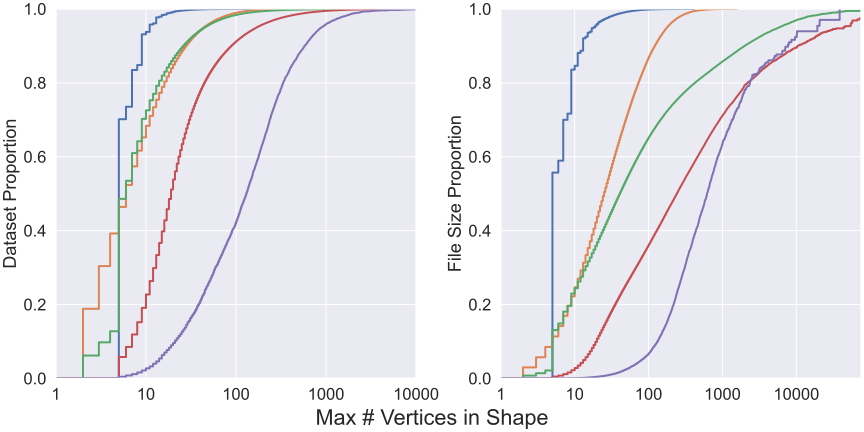
\includegraphics[width=14.5cm]{images/data_distrb_all.png}
    \caption{Cumulative distribution of the vertex count for the geometries based on the dataset. The right plot is weighted by the number of vertices, indicating how the overall size is distributed. For example, the size of one shape containing 30 vertices is equal to 6 shapes containing 5 vertices.}
        \label{img:data_distrb_all}
\end{figure}

%För varje:
%Antal punkter avg
%Tot points, avg points per shape
%https://texblog.org/2017/02/06/proper-tables-with-latex/
%https://tex.stackexchange.com/questions/380233/how-to-manually-make-tables-using-booktabs





\subsection{Intersection Data}
\label{sec:intersectiondataintro}
In order to benchmark the operations of intersection, datasets consisting of pairs of shapes resulting in the different cases of intersection are needed.

\subsubsection{OSM \& GADM}
The common case for intersection, if picking two geometries at random, is that no intersection occurs. To collect the queries of interest, the bounding boxes of all shapes were pairwise tested for intersection, and the queries containing an intersection were kept. In addition to the case of \emph{no intersection}, the possible distinct cases when the bounding boxes intersect are \emph{no intersection}, \emph{intersection with crossing segments}, and \emph{intersection by contains}.

The testing was performed for all shapes in \emph{Admin Borders}, for all shapes of type building or highway (used for identifying any kind of road, street or path) in the city of Lund (subset of \emph{Sweden All}), and random subsets of 100 000 queries from \emph{Sweden All} and \emph{China Water}.

\subsubsection{Manually Created Special Cases}
Since the shapes can consist of polylines, polygons, polygons with holes, and multipolygons, there exist numerous possible relations between the types of the intersecting shapes. Furthermore, a number of edge cases, such as shapes consisting of parallel lines, have to be accounted for when implementing intersection. In order to test for those, along with the possible worst- and best-case scenarios, the GIS editing tool \emph{QGIS} was used to manually create a dataset of such shapes.

\section{Validation \& Benchmarking Environment}
A test bench was created in order to evaluate and verify the different implementations of compression algorithms and their operations. Due to Python's large number of existing modules and community support, the test bench was written as a Python \emph{Jupyter Notebook}. By being able to split code into cells and have the output from each cell presented directly under the code, Jupyter Notebooks can be used to present both code and plots of results in a structured manner.
\\\\
To allow for fast integration of new or altered algorithm implementations, the test bench was written in a generalized manner, being as decoupled from the algorithm implementation as possible. This was achieved by having an abstract base class that consists of the methods for compression, decompression, and the corresponding operations. Each algorithm derives from the base class and provides implementations of the abstract methods. With this setup, a new algorithm can be added by simply changing one line in the test bench. Furthermore, the dataset used in the benchmarking can also be specified by changing one configuration variable.

%https://docs.google.com/viewer?a=v&pid=sites&srcid=ZGVmYXVsdGRvbWFpbnx0ZXN0MTIzNHNpbTQ2NXxneDpiYTJmYWIwYTAyOGJiZmQ
\subsection{Validation of Operations}
Test-driven development is a common strategy used to maintain system correctness over time. By shortening the feedback loop in the form of automated testing, bugs in implementations can be caught in a matter of seconds \cite{tdd}.

For lossless compression algorithms, one obvious test case is verifying that the decompressed data is equal to the original data. When dealing with geometric data, it is also the case that all operations should exhibit the same behavior in the geometry space, regardless of the algorithm used. When modifying geometries, one way to validate operation correctness is to perform the operation on the compressed data using the untested algorithm and then decompress the data altogether and compare the output with a trusted implementation.
\\\\
To ensure the correctness of the implemented algorithms in the thesis, a validation section is included in the test bench. During benchmarking, each query and its corresponding result are logged. After executing all queries, the queries are re-run using a verified implementation, and the outputs are compared to ensure consistency.

\subsection{Shapely}
Comparison fairness is essential when benchmarking different compression algorithms. Therefore, all algorithms assume the same input and output format. The Python GEOS library \emph{Shapely} is used as the algorithms' start and end point format. Shapely comes with a spatial data model supporting common functionalities. The premise of Shapely is its convenience for working with and operating on spatial objects without the need for relational databases \cite{shapely}.

All the geometries described in the theoretical background, such as Point, LineString, Polygon, and MultiPolygon, are available as geometric Python objects supporting various spatial operations. Additionally, Shapely is compatible with common formats, such as WKT, WKB, and GeoJSON, making working with online datasets convenient \cite{shapely}.

\begin{figure}[htbp]
    \centering
    \includesvg[width=15cm]{images/Benchmarking diagram.svg}
    \caption{Visualization overview of the benchmarking pipeline. Orange boxes indicate values passed to benchmarking or validation and \textit{ALG} is the current  algorithm to test.}
    \label{img:bench}
\end{figure}

\subsection{Benchmarking}
For benchmarking the algorithms, it is assumed that all the input data for the algorithms are stored in RAM, and benchmarking does not include the overhead of reading and writing data to storage. This enhances a fair comparison by removing the impact on performance caused by the storage solution. The compression, decompression, and operations assume three different starting and ending premises:
\begin{itemize}
    \item \textbf{Compress: }Shapely object $\xrightarrow{output}$ Binary String  
    \item \textbf{Decompress: }Binary String $\xrightarrow{output}$ Shapely Object    
    \item \textbf{Operations: }Binary String $\xrightarrow{output}$ Value/Binary String
\end{itemize}

Since the third-party library Shapely is used for the algorithms, consistency of its use between the different algorithms must be considered. For instance, there are various ways of instantiating Shapely objects. Suppose that different Shapely object creation strategies are used for different algorithms. In that case, the benchmarking comparison might be unfair since the relative efficiency differences between the methods in the third-party library are unknown.

The common benchmarks for compression, decompression, and operations are running time. For compression and decompression, the size differences in bytes for the different algorithms are also investigated.  In Figure \ref{img:bench}, the pipeline for benchmarking the algorithms can be seen.


% \todo{större text, ta bort att tid mäts i operations. Döpa om "operations" till Validation?}


\subsection{Performance Profiling}Due to Python being an interpreted language and lacking an optimizing compiler, profiling is essential for finding implementation bottlenecks. The Python profiling tool \emph{Kernprof}, together with its complement \emph{line\_profiler}, can be used to extract line-by-line statistics for different functions. For each line, the statistics contain the number of hits, the accumulated execution time, and its corresponding time percentage relative to the encapsulating function \cite{kernprof}.

In addition to locating slow code, profiling provides algorithmic insight. When developing algorithms, understanding which parts are logically flawed or time-consuming is valuable for creating efficient and robust algorithms. 
%compress: shapely -> bin, decomp: bin -> shapely, %operations: bin -> value/bin
%Avoid file reading/writing part of time. %To/from_ragged_array in Shapely for consistency


